\documentclass[a4paper,12pt,oneside]{article}

\usepackage[utf8]{inputenc}
\usepackage[T2A]{fontenc}
\usepackage[russian]{babel}
\usepackage[usenames]{xcolor}
\usepackage{etoolbox}
\usepackage{listings}
\usepackage{graphicx}
\usepackage{cmap}
\usepackage{indentfirst}
\usepackage{makeidx}
\usepackage[unicode]{hyperref}

\newif\ifanswers
\answerstrue

\hypersetup{
%bookmarks=true,            % show bookmarks bar?
%unicode=false,             % non-Latin characters in Acrobat’s bookmarks
pdfproducer={Producer},    % producer of the document
pdfkeywords={keywords},    % list of keywords
pdfnewwindow=true,         % links in new window
colorlinks=true,           % false: boxed links; true: colored links
linkcolor=black,           % color of internal links
citecolor=black,           % color of links to bibliography
    filecolor=black,           % color of file links
    urlcolor=black             % color of external links
}

\renewcommand{\rmdefault}{cmr} 

\renewcommand{\texttt}[2][black]{\textcolor{#1}{\ttfamily #2}}

\renewcommand\floatpagefraction{0.8} %% default value: 0.5
\renewcommand\topfraction{0.8}       %% default value: 0.7

\definecolor{OliveGreen}{cmyk}{0.64,0,0.95,0.40}
\definecolor{mauve}{rgb}{0.58,0,0.82}

\setlength{\parskip}{6pt}

\makeindex

\title{Лекция по Toolchain}
\author{
  Владимиров Константин Игоревич\\
  \texttt{konstantin.vladimirov@gmail.com}
}
\date{\today}

\lstset{
language=C++,                           % Code langugage
basicstyle=\ttfamily,                   % Code font, Examples: \footnotesize, \ttfamily
keywordstyle=\color{OliveGreen},        % Keywords font ('*' = uppercase)
commentstyle=\color{gray},              % Comments font
stringstyle=\color{mauve},
numbers=left,                           % Line nums position
numberstyle=\tiny,
numbersep=10pt,
stepnumber=1,                           % Step between two line-numbers
frame=none,                             % A frame around the code
tabsize=2,                              % Default tab size
captionpos=b,                           % Caption-position = bottom
breaklines=true,                        % Automatic line breaking?
breakatwhitespace=false,                % Automatic breaks only at whitespace?
showspaces=false,                       % Dont make spaces visible
showstringspaces=false,
showtabs=false,                         % Dont make tabls visible
columns=flexible,                       % Column format
title=\lstname,
caption={},
extendedchars=\true,
inputencoding=utf8,
}

\begin{document}

\tableofcontents

\pagebreak
\section{Toolchain}\label{Toolchain}

Общеупотребительным англицизмом toolchain (можно перевести как ``набор средств разработки'' или как ``система компиляции'', можно оставить просто слово ``тулчейн'') обозначают набор средств разработки, совместно используемых для создания программного обеспечения. Обычно это компилятор, ассемблер, линкер, а также набор бинарных утилит. Иногда в состав toolchain включают средства отладки и верификации программ, профилировщики и анализаторы покрытия кода.

\subsection{Обзор средств разработки}\label{Overview}

Обычно весь набор средств разработки скрыт от пользователя за единой программой-драйвером (как в случае GNU Toolchain когда роль такой программы играет GCC) или за ширмой средств IDE (как в случае Microsoft Toolchain, когда компиляция ассемблирование и сборка происходят по нажатию кнопки F7 в Visual Studio).

Кроме GNU и Microsoft, известны также LLVM toolchain, Intel toolchain, ARM toolchain а также пакеты средств разработки Borland и Comeau. Для всех примеров ниже будет использоваться GNU Toolchain, но иногда будут приводиться примеры из других средств разработки, там, где есть некие концептуальные отличия. Точно также ниже будут описаны в основном примеры компиляции программ на языке C, разве что с некоторыми экскурсиями в C++ и Fortran.

Эта лекция ставит перед собой следующие цели:

\begin{itemize}
\item Сделать ясной структуру и последовательность работы системы компиляции в целом
\item Осветить роль каждого из инструментов в отдельности, его применимость и решаемые им задачи
\item Дать базу для самостоятельных экспериментов (на примере GNU Toolchain)
\item Изложить основные этапы портирования toolchain на новую архитектуру
\end{itemize}

Первый пункт можно переформулировать как простой и конкретный вопрос: что происходит при исполнении строчки вида

\begin{verbatim}
$ gcc test.c
\end{verbatim}

Правильный ответ: происходит запуск трёх основных программ, как это показано на (рис. \ref{fig:simplified_scheme}).

\begin{figure}[ht]
\centering
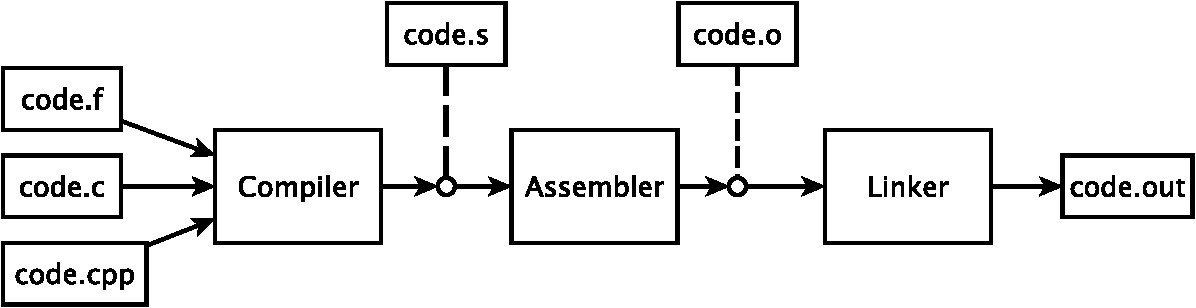
\includegraphics[width=1.0\textwidth]{illustrations/simplified-scheme-crop.pdf}
\caption{Упрощенная схема toolchain}
\label{fig:simplified_scheme}
\end{figure}

\begin{enumerate}
\item \textbf{Компилятор} -- в случае GNU toolchain это cc1 или cc1plus для кода на C или C++, в случае MSVS это cl.exe. Переводит текст на языке высокого уровня в язык ассемблера целевой архитектуры
\item \textbf{Ассемблер} -- в случае GNU toolchain это as, в случае MSVS это ml.exe. Кодирует ассемблер целевой архитектуры и порождает объектный код
\item \textbf{Линкер} -- в случае GNU toolchain это ld или gold, в случае MSVS это link.exe. Собирает несколько объектных модулей в исполняемый файл
\end{enumerate}

Toolchain не исчерпывается этой упрощенной схемой, но для начала рассмотрение трёх основных компонент позволяет создать общую картину происходящего.

\subsection{Компилятор}

Компилятор является главным и наиболее известным компонентом средств разработки (автору не раз доводилось слышать как ``компилятором'' называют и драйвер и весь toolchain). Тем не менее, происходящее внутри компилятора часто также остается неизвестным разработчику, как и происходящее внутри системы компиляции в целом.

\begin{figure}[ht]
\centering
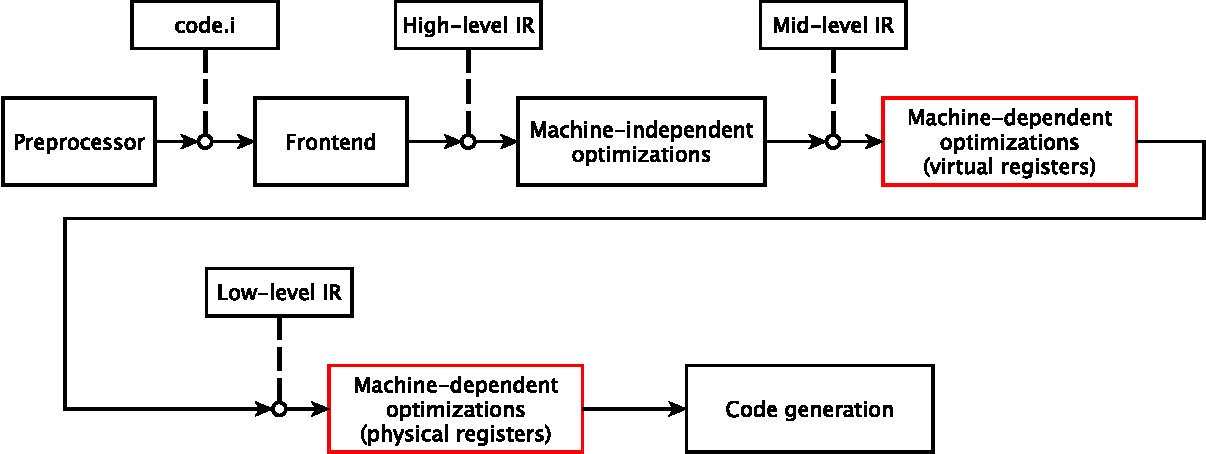
\includegraphics[width=1.0\textwidth]{illustrations/compiler-crop.pdf}
\caption{Компилятор изнутри}
\label{fig:compiler_scheme}
\end{figure}

На (рис. \ref{fig:compiler_scheme}) изображена схема работы компилятора, состоящая из следующих элементов:

\begin{enumerate}
\item \textbf{Препроцессор} -- занимается текстовой обработкой исходного текста и подготовкой к компиляции
\item \textbf{Фронтенд} -- переводит язык высокого уровня в промежуточное представление
\item \textbf{Бэкенд} -- состоит из оптимизаций на разных уровнях промежуточного представления и кодогенерации в ассемблер целевой архитектуры. Иногда его делят на middle-end, где выполняются машинно-независимые оптимизации и backend (выделен красным цветом), где происходят машинно-зависимые преобразования.
\end{enumerate}

В LLVM toolchain, препроцессор и фронтенд вынесены в отдельную программу (clang), которая порождает машинно-независимое промежуточное представление (intermediate representation или для краткости IR) над которым сосбтвенно компилятор llvm производит преобразования до ассемблера. Кроме того собственно препроцессор часто поставляет отдельно в наборе бинарных утилит, например в составе GNU Toolchain программа, производящая препроцессинг называется cpp. Она, тем не менее, не запускается в нормальной циклограмме работы, так как препроцессор является частью компилятора cc1, а cpp это просто отдельно лежащий препроцессор, отпиленный для удобства.

\subsubsection{Препроцессор}

Работа препроцессора происходит в основном над текстом и в случае языка C регламентирована стандартом языка (5.1.1.2 в C11). В случае gcc, для препроцессирования файла имеется опция -E.

\begin{figure}[ht]
\centering
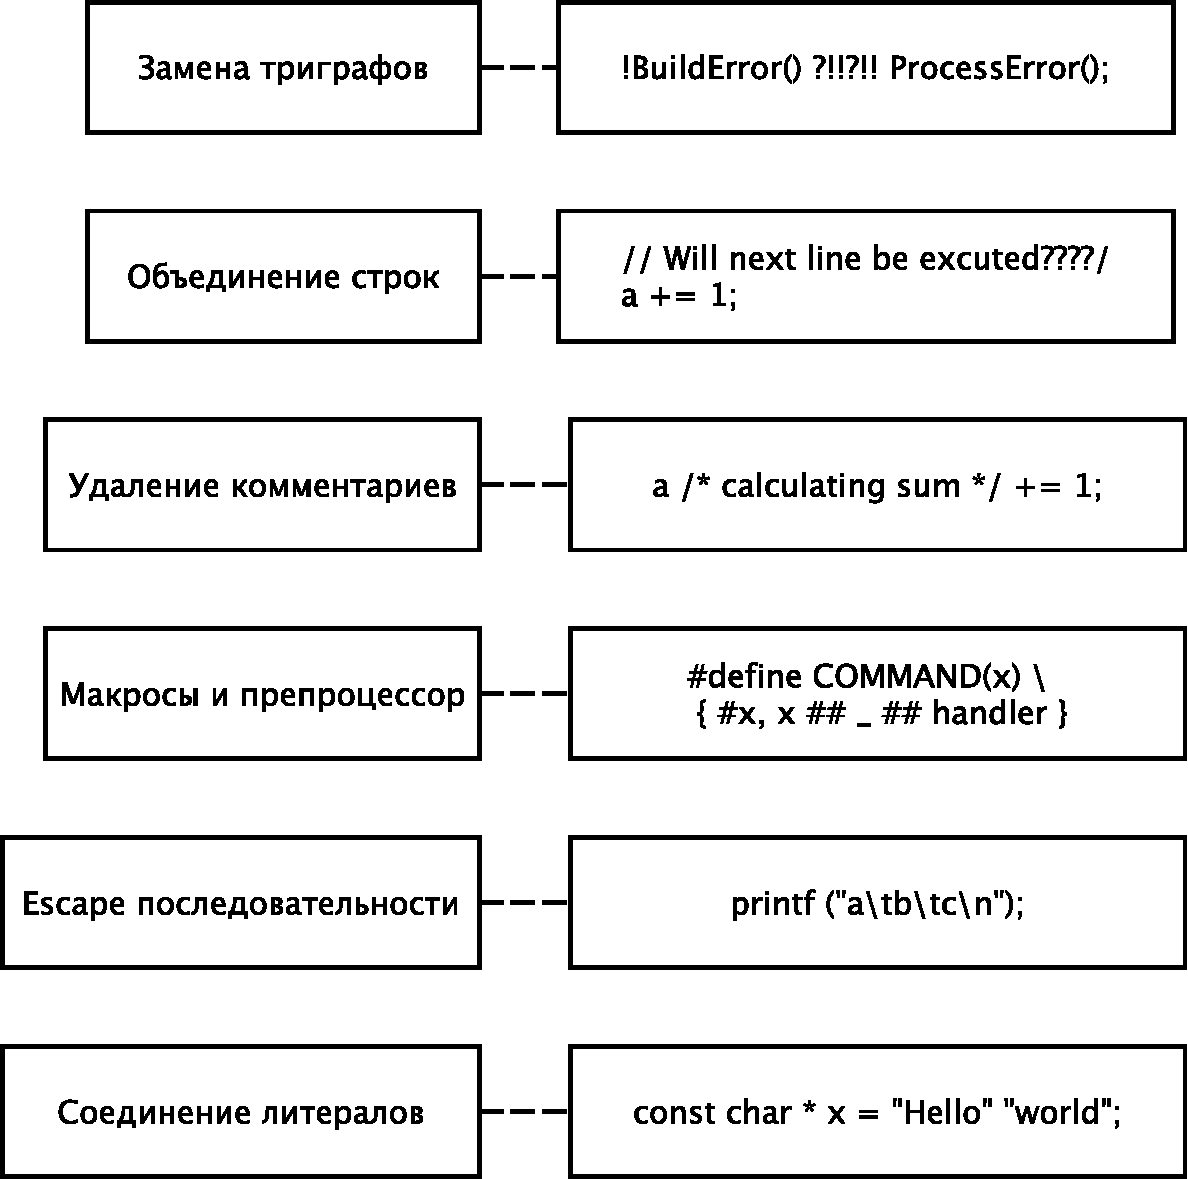
\includegraphics[width=0.8\textwidth]{illustrations/preprocessor-scheme-crop.pdf}
\caption{Схема препроцессора}
\label{fig:preproc_scheme}
\end{figure}

Препроцессор, как это изображено на (рис. \ref{fig:preproc_scheme}) выполняет действия в следующем порядке:

\begin{itemize}
\item Замена триграфов.
Например попробуйте понять что происходит на этой строчке: \lstinline$!ErrorOccured() ??!??! HandleError();$. Правильный ответ -- здесь вместо вертикальной черты использован триграф \lstinline$??!$ так что непонятная мешанина знаков в середине это просто длинное или. Ещё пример: 

\begin{lstlisting}
// WTF????/
a += 1;
\end{lstlisting}

Здесь использован триграф \lstinline$??/$, обозначающий обратный слеш. Что приводит к следующему пункту.
\item Объединение строк по обратному слешу
В примере выше после раскрытия триграфа остаётся:
\begin{lstlisting}
// WTF??\
a += 1;
\end{lstlisting}
И на этом этапе эти строки будут объединены в:
\begin{lstlisting}
// WTF??a += 1;
\end{lstlisting}
\item Разбиение на токены препроцессирования и замена комментариев пробелами
Здесь будут вычеркнуты все комментарии и заменены одним пробельным символом.
\item Раскрытие макросов и обработка директив препроцессора
На этом этапе раскрываются все макро-определения, как явно введенные через директиву \lstinline!#define! так и неявно заданные как билтины компилятора (скажем \lstinline!__cplusplus! позволяющий отличить компиляцию на C и C++). В случае GNU Toolchain, посмотреть встроенные макроопределения можно с помощью опций -E -dM.
\item Замена escape-последовательностей
Я полагаю, все встречались со \lstinline!\n! или \lstinline!\t! при использовании функции \lstinline!printf!
\item Соединение стоящих рядом строковых литералов
\end{itemize}

Файл, получившийся после препроцессирования, называется единицей трансляции (translation unit) и обрабатывается компилятором. В некоторых языках (например Fortran) несколько единиц трансляции могут располагаться в одном файле.

\subsubsection{Фронтенд}

Фронтенд компилятора работает с препроцессированным файлом и выполняет тяжелую задачу разбора языковых конструкций и перевода программы с конкретного языка программирования (например C++) в высокоуровневое промежуточное представление, удобное для машинно-независимых оптимизаций. Обычно фронтенд осуществляет:

\begin{itemize}
\item Лексический анализ: выделение ключевых слов языка, имён переменных и символов операций
Пример: \lstinline!int z = x+++y;! будет распознано как \lstinline!int z = (x++)+y;! (слева направо) но при этом \lstinline!int z = x = y;! будет распознано как \lstinline!int z = (x = y);! (справа налево)
\item Синтаксический анализ и построение дерева синтаксического разбора (см. пример на рис. \ref{fig:ast_scheme})
\item Анализ и вывод типов выражений
\end{itemize}

\begin{figure}[ht]
\centering
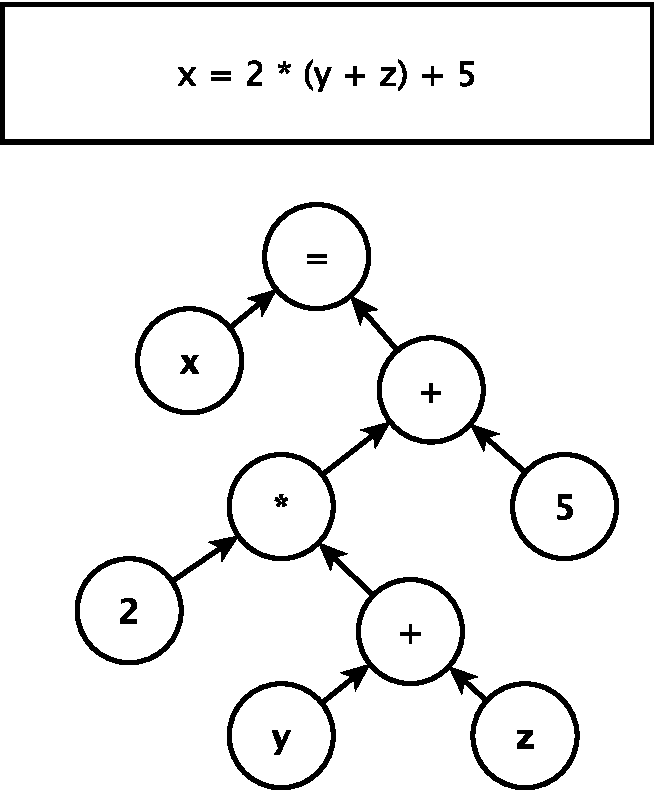
\includegraphics[width=0.5\textwidth]{illustrations/ast-example-crop.pdf}
\caption{Дерево синтаксического разбора}
\label{fig:ast_scheme}
\end{figure}

Иногда фронтенду приходится решать довольно сложные задачи связанные с тем, что современные языки высокого уровня (такие как C++) могут иметь неочевидный синтаксис и семантику.

Классический пример:

\begin{lstlisting}
ifstream datafile ("ins.dat");
list<int> data (istream_iterator<int>(dataFile),
                istream_iterator<int>());
\end{lstlisting}

Может показаться удивительным, но вторая строчка содержит объявление функции, а вовсе не заполнение контейнера из файла. Спасает простановка скобок:

\begin{lstlisting}
ifstream datafile ("ins.dat");
list<int> data ((istream_iterator<int>(dataFile)),
                istream_iterator<int>());
\end{lstlisting}

Ещё один пример:

\begin{lstlisting}
template <class T>
foo (T x)
{
  T::iterator *y;
  /* .... */
}
\end{lstlisting}

Увы, без дополнительных подсказок, синтаксический разбор определяет это как умножение некоего статического члена \lstinline!T::iterator! на некоторую глобальную переменную \lstinline!y!. Чтобы помочь фронтенду, здесь уместно добавить ключевое слово \lstinline!typename!:

\begin{lstlisting}
template <class T>
foo (T x)
{
  typename T::iterator *y;
  /* .... */
}
\end{lstlisting}

Как правило, результатом работы фронтенда является промежуточное представление (Gimple в случе GCC, LLVM IR в случае LLVM и так далее).

\subsubsection{SSA представление}

SSA это аббревиатура для static single assignment. Программа считается представленной в SSA-форме, если каждой именованной переменной в программе может быть только один раз присвоено значение. Одним из важных следствий этого определения является referencial transparency -- то свойство программы, когда значение переменной независимо от её положения в программе.

\begin{lstlisting}
x = 1;
y = x + 1;
x = 2;
z = x + 1;
\end{lstlisting}

Эта программа является корректным кодом на C, но значение \lstinline!x! зависит от анализируемой строчки, в результате чего \lstinline!y = x + 1! и \lstinline!z = x + 1! имея идентичную форму определения, имеют разные значения. В случае SSA-формы этот код может быть переписан:

\begin{lstlisting}
x1 = 1;
y = x1 + 1;
x2 = 2;
z = x2 + 1;
\end{lstlisting}

Здесь очевидно, что разные значения соответствуют разной форме определения. Но для линейных участков всё просто. Сложнее преобразовать в SSA форму ветвления. Например:

\begin{lstlisting}
x = input ();
if (x > 42)
  y = 1;
else
  y = x - 2;
use (y);
\end{lstlisting}

Здесь для того, чтобы избавиться от двух определений \lstinline!y! нужно ввести $\phi$-функцию которая будет ``выбирать'' верное значение \lstinline!y! из двух пришедших к ней $y_1$ и $y_2$ как показано на рисунке:

\begin{figure}[h!]
\centering
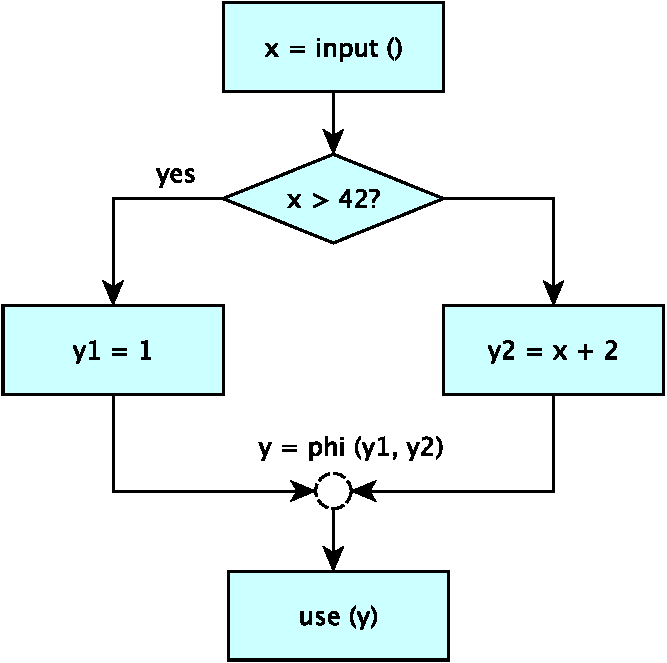
\includegraphics[width=0.6\textwidth]{illustrations/ssa-romb-crop.pdf}
\caption{$y = \phi(y_1, y_2)$}
\label{fig:ssa_romb_scheme}
\end{figure}

Изначально такие функции получили своё название от phony-functions (фальшивые функции), но название прижилось и сократилось. Обозначения \lstinline!phi(y1, y2)! и $\phi(y_1, y_2)$ далее будут достаточно свободно взаимозаменяемы.

К сожалению, их никак нельзя переписать на C, но в GIMPLE дампах они выглядят так:

\begin{lstlisting}
  <bb 3>:
  # n_5 = PHI <5(2), _6(4)>
  # mult_acc_7 = PHI <1(2), mult_acc_8(4)>
...
\end{lstlisting}

Эта запись означает, что есть два пути, по которым управление сходится в \lstinline!bb3! из блоков \lstinline!bb2! (там где в скобках стоит 2) и \lstinline!bb4! для \lstinline!n_5!, причём внутри \lstinline!bb2! определение этой переменной имеет имя \lstinline!5! (по правилам GIMPLE это просто константа 5), а в \lstinline!bb4! имеет имя \lstinline!_6! (искуственно созданные временные переменные в GIMPLE часто имеют безликие имена \lstinline!_1!, \lstinline!_2! и так далее).

\subsubsection{Машинно-независимые преобразования}

Для примера работы промежуточного представления можно рассмотреть функцию, вычисляющую (с первого взгляда -- крайне неоптимально) факториал числа, переданного в качестве аргумента.

\begin{lstlisting}
unsigned
fact (unsigned x)
{
  if (x < 2)
    return 1;

  return x * fact (x-1);
}
\end{lstlisting}

Трансформации сильно зависят от опций конкретного компилятора, рассмотрим этот пример как скомпилированный с \lstinline!-O2! в 64-битном режиме (обычно чем выше уровень, тем сильнее оптимизация, уровень 2 означает применять большинство полезных оптимизаций и оптимизировать код по скорости исполнения).

После работы фронтенда GCC, эта функция представлена в виде машинно-независимого языка промежуточного представления GIMPLE. В виде графа её можно изобразить как показано на рис. \ref{fig:fact_gimple_ssa}.

\begin{figure}[ht]
\centering
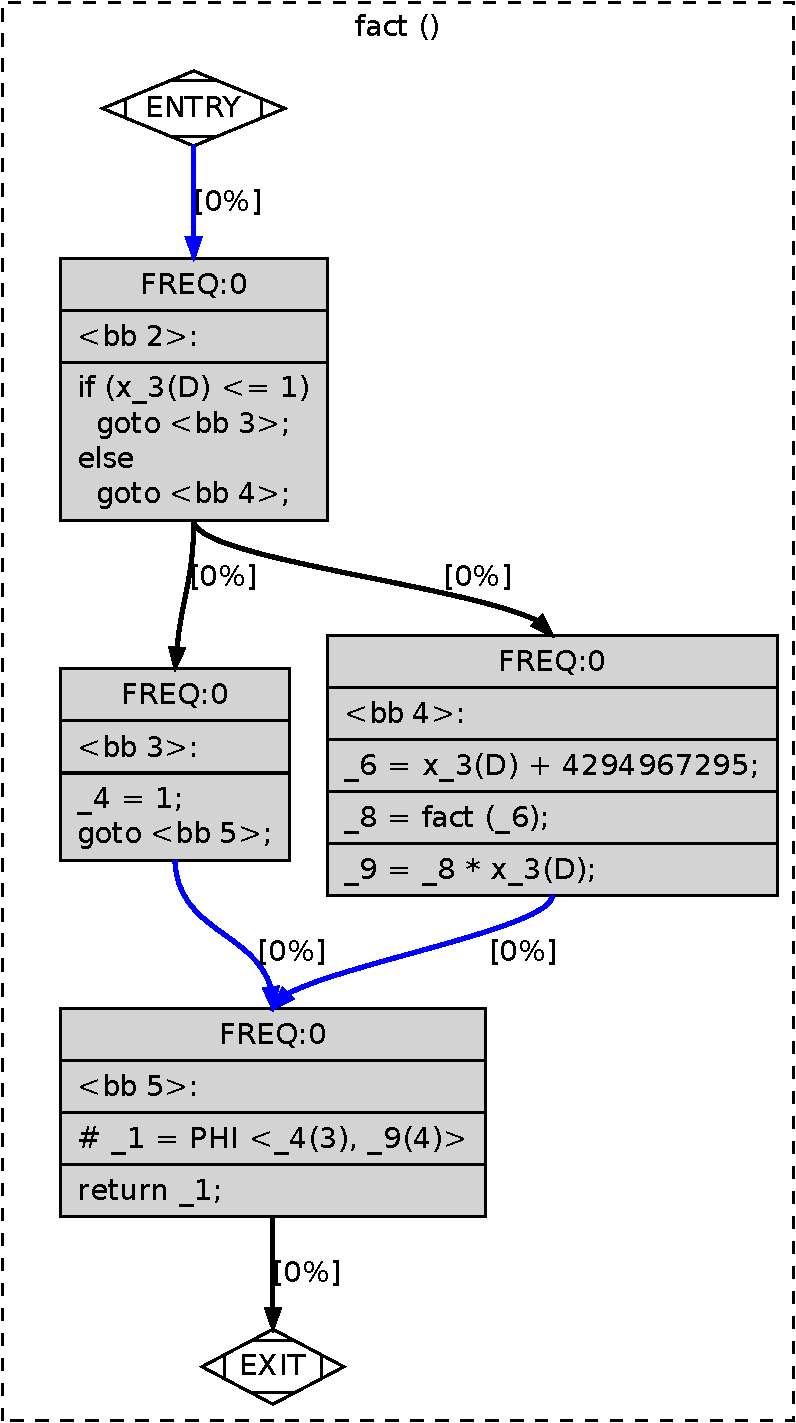
\includegraphics[width=0.5\textwidth]{illustrations/fact-ssa-crop.pdf}
\caption{GIMPLE на начальных фазах}
\label{fig:fact_gimple_ssa}
\end{figure}

Для получения дампа, можно воспользоваться опцией \lstinline!-fdump-tree-ssa! а в общем случае опцией \lstinline!-fdump-tree-all! позволит посмотреть все результаты работы всех фаз на уровне GIMPLE.

Программа на рис. \ref{fig:fact_gimple_ssa} практически повторяет структуру исходного кода на C, с учётом перевода в SSA и расстановки $\phi$-функций. Далее за дело берутся машинно-независимые оптимизации, которых в GCC 5.2 насчитывается более двухсот. Уже через несколько итераций происходит подстановка хвостового вызова и код начинает выглядет гораздо интереснее, как показано на (рис. \ref{fig:fact_gimple_release_ssa}).

\begin{figure}[ht]
\centering
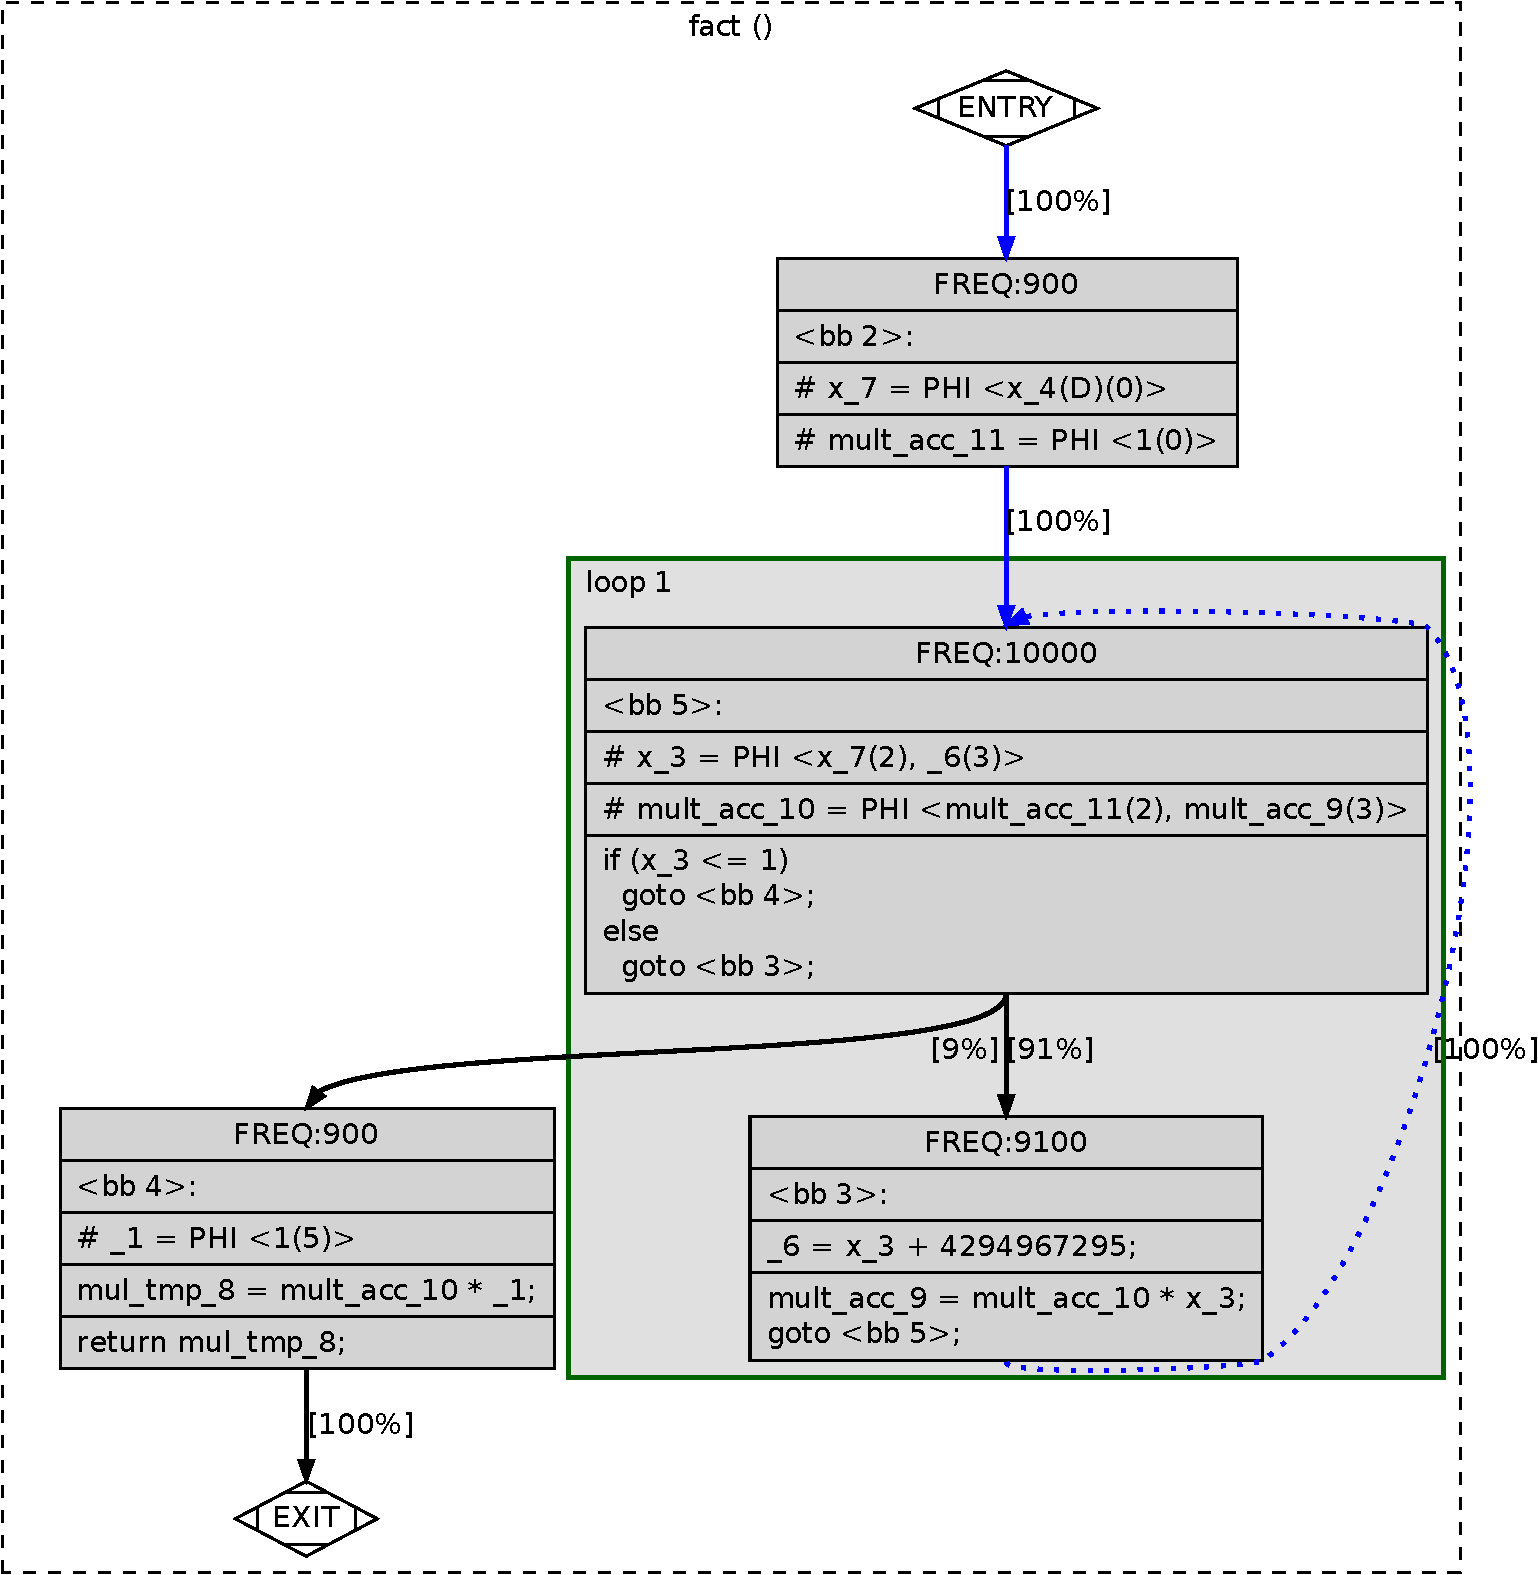
\includegraphics[width=0.9\textwidth]{illustrations/fact-release_ssa-crop.pdf}
\caption{GIMPLE после tail-call оптимизаций}
\label{fig:fact_gimple_release_ssa}
\end{figure}

Пунктирной линией показана обратная дуга цикла, который получился в результате раскрытия хвостовой рекурсии. Кроме того, следует обратить внимание на расставленные вероятности переходов -- здесь они расставлены компилятором априорно. Их можно сделать гораздо более точными если использовать при компиляции профиль реального запуска программы.

\subsubsection{Машинно-зависимые преобразования}

После окончания машинно-независимых преобразований, код переводится в машинно-зависимую форму, называемую в случае GCC register transfer language или RTL. Интересно, что этот перевод называется по разному в разных компиляторах. В мире LLVM говорят ``lowering'' выражая этим понижение уровня представления. В мире GCC говорят ``expand'' -- раскрытие машинно-независимых конструкций в машинно-зависимый формат.

Все инструкции в машинно-зависимом формате зависят от описания конкретной машины в бэкенде компилятора и на ранних фазах RTL оперируют с виртуальными регистрами. Виртуальные регистры это не SSA представление, это абстрактная регистровая машина, в которой количество регистров не ограничено.

Получить дампы RTL в GCC можно с помощью опции \lstinline!-fdump-rtl-all!, где, как обычно, вместо all можно подать символическое имя фазы (\lstinline!-fdump-rtl-expand! для кода сразу после раскрытия и так далее).

Чтение дампов RTL осложняется тем фактом, что они представлены в сложном LISP-подобном формате:

\begin{verbatim}
(insn 15 14 16 5 (parallel [
            (set (reg:SI 90 [ D.1850 ])
                (mult:SI (reg:SI 90 [ D.1850 ])
                    (reg/v:SI 92 [ x ])))
            (clobber (reg:CC 17 flags))
        ]) -1
     (nil))
\end{verbatim}

На самом деле выше происходит следующее: в виртуальный регистр с номером 90 записывается произведение виртуальных регистров 90 и 92, параллельно с чем непредсказуемо изменяется флаговый регистр. Для простоты это можно записать как:

\begin{lstlisting}
v90 = v90 * v92;
clobber (v17);
\end{lstlisting}

Здесь буква v подчеркивает, что регистры виртуальные. На рис. \ref{fig:fact_rtl_expand} изображен код факториала сразу после раскрытия в машинно-зависимый формат.

\begin{figure}[htb]
\centering
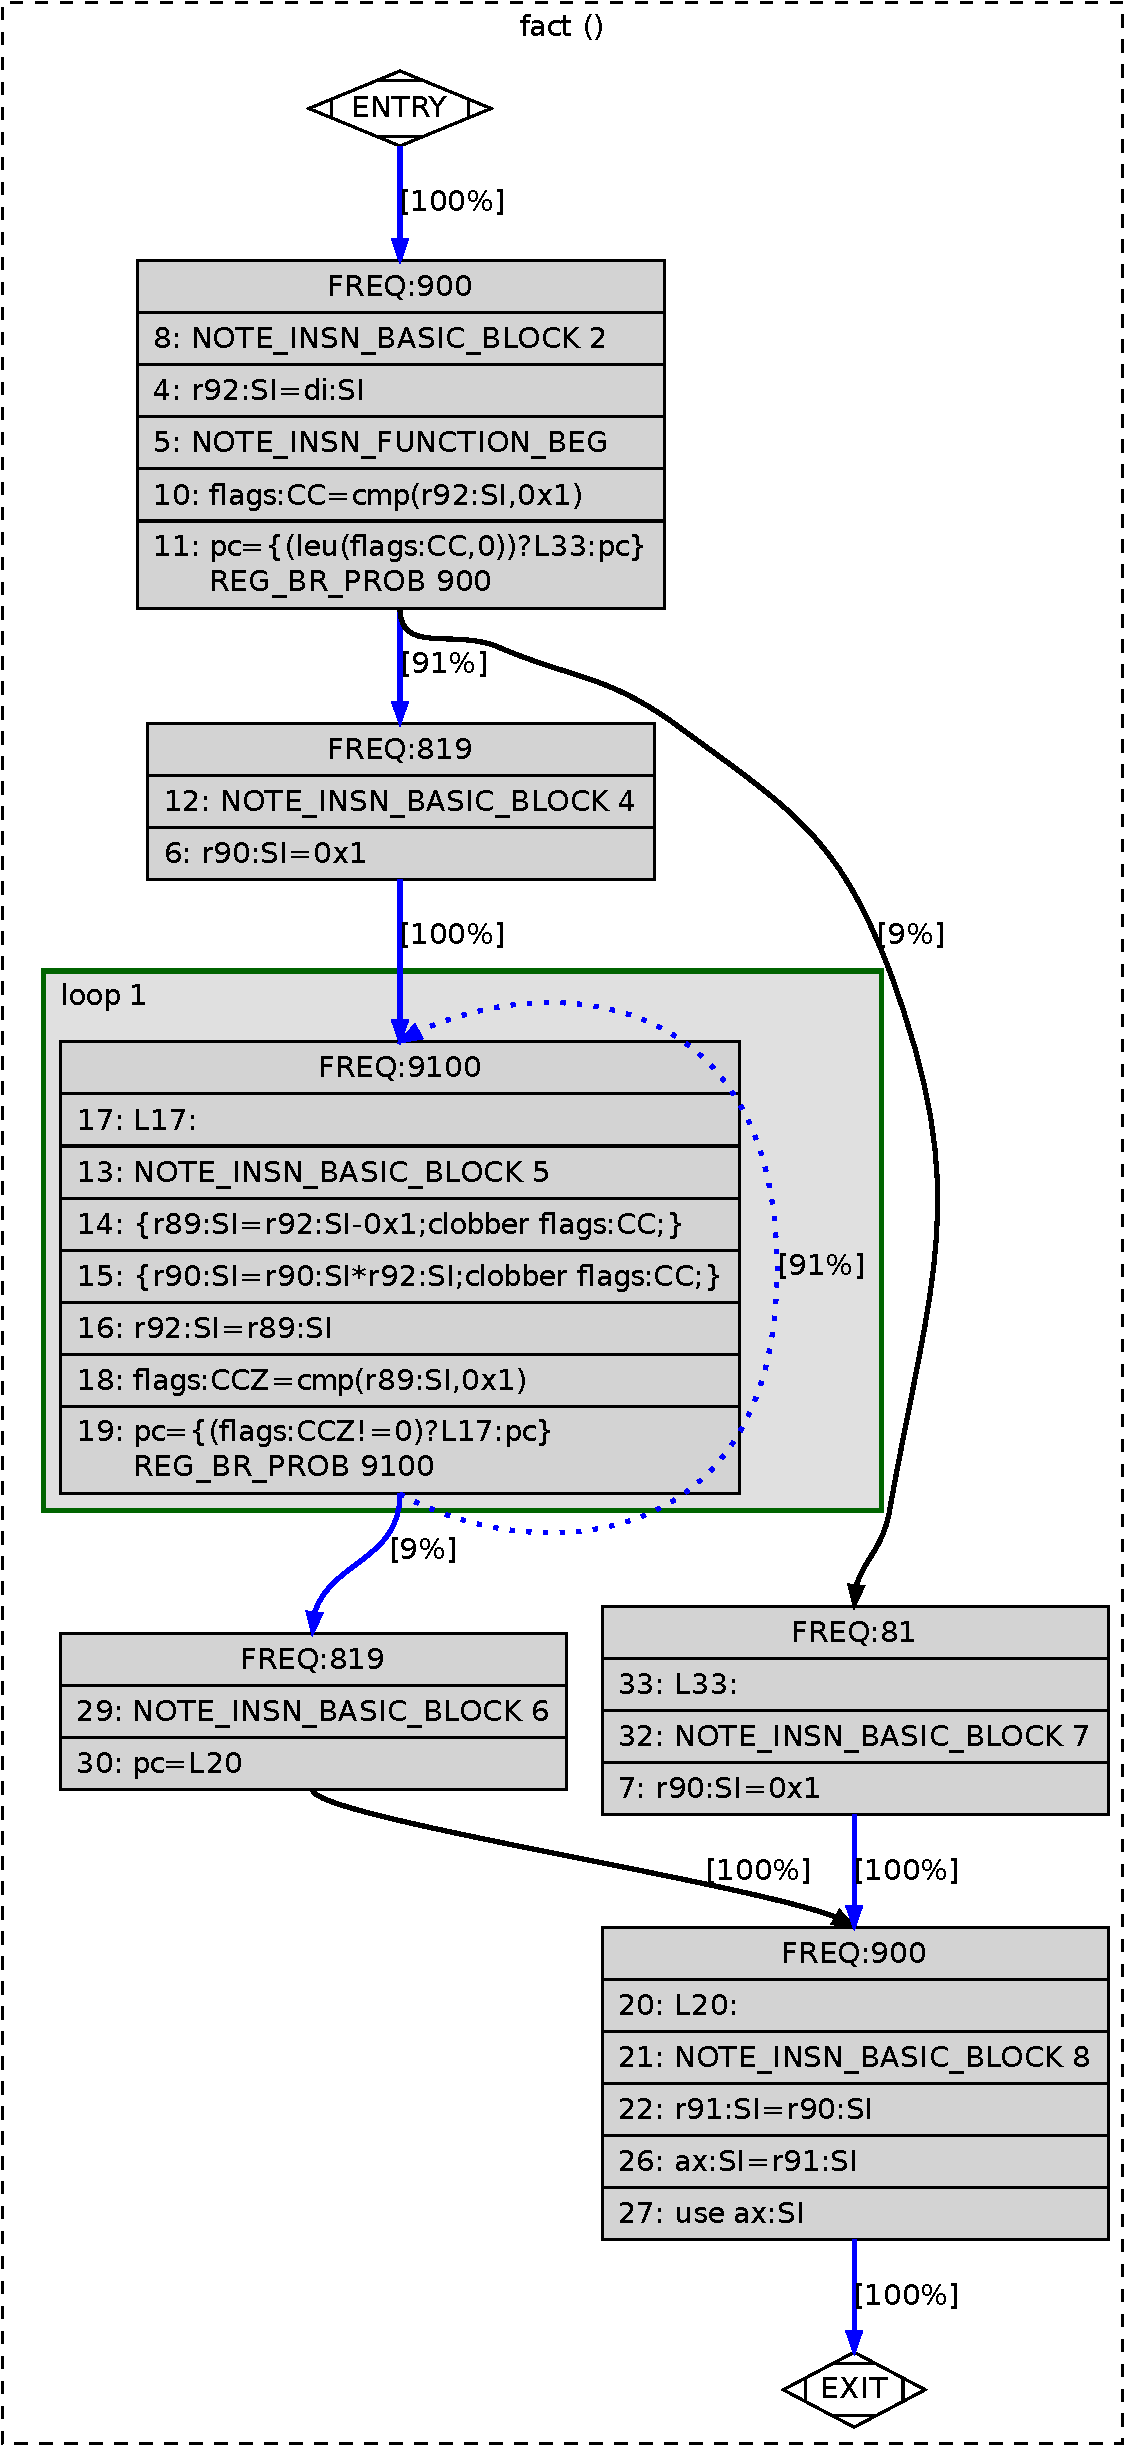
\includegraphics[height=0.7\textheight]{illustrations/fact-expanded-crop.pdf}
\caption{RTL с виртуальными регистрами}
\label{fig:fact_rtl_expand}
\end{figure}

Можно заметить, что каждому регистру сопоставлен режим (register mode) в котором он используется. Некоторые из этих режимов перечисленны ниже:

\begin{enumerate}
\item SI -- одно машинное слово (single integer mode). Обычно соответствует 32 битам.
\item DI, HI, QI -- двойное слово, половинное и четверть слова (double, half, quad)
\item CC, CCZ -- регистры флагов
\end{enumerate}

Использование регистра в каком-то режиме не отменяет того, что после окончания жизни этой переменной он не будет переиспользован в каком-то другом режиме.

После выполнения преобразований на виртуальных регистрах, должен отработать распределитель регистров, который отображает виртуальные регистры в физические регистры, заданные в описании целевой архитектуры. Для x86 это ax, bx, cx, dx и так далее. Пример RTL с физическими регистрами приведен на рис \ref{fig:fact_rtl_reload}

\begin{figure}[htb]
\centering
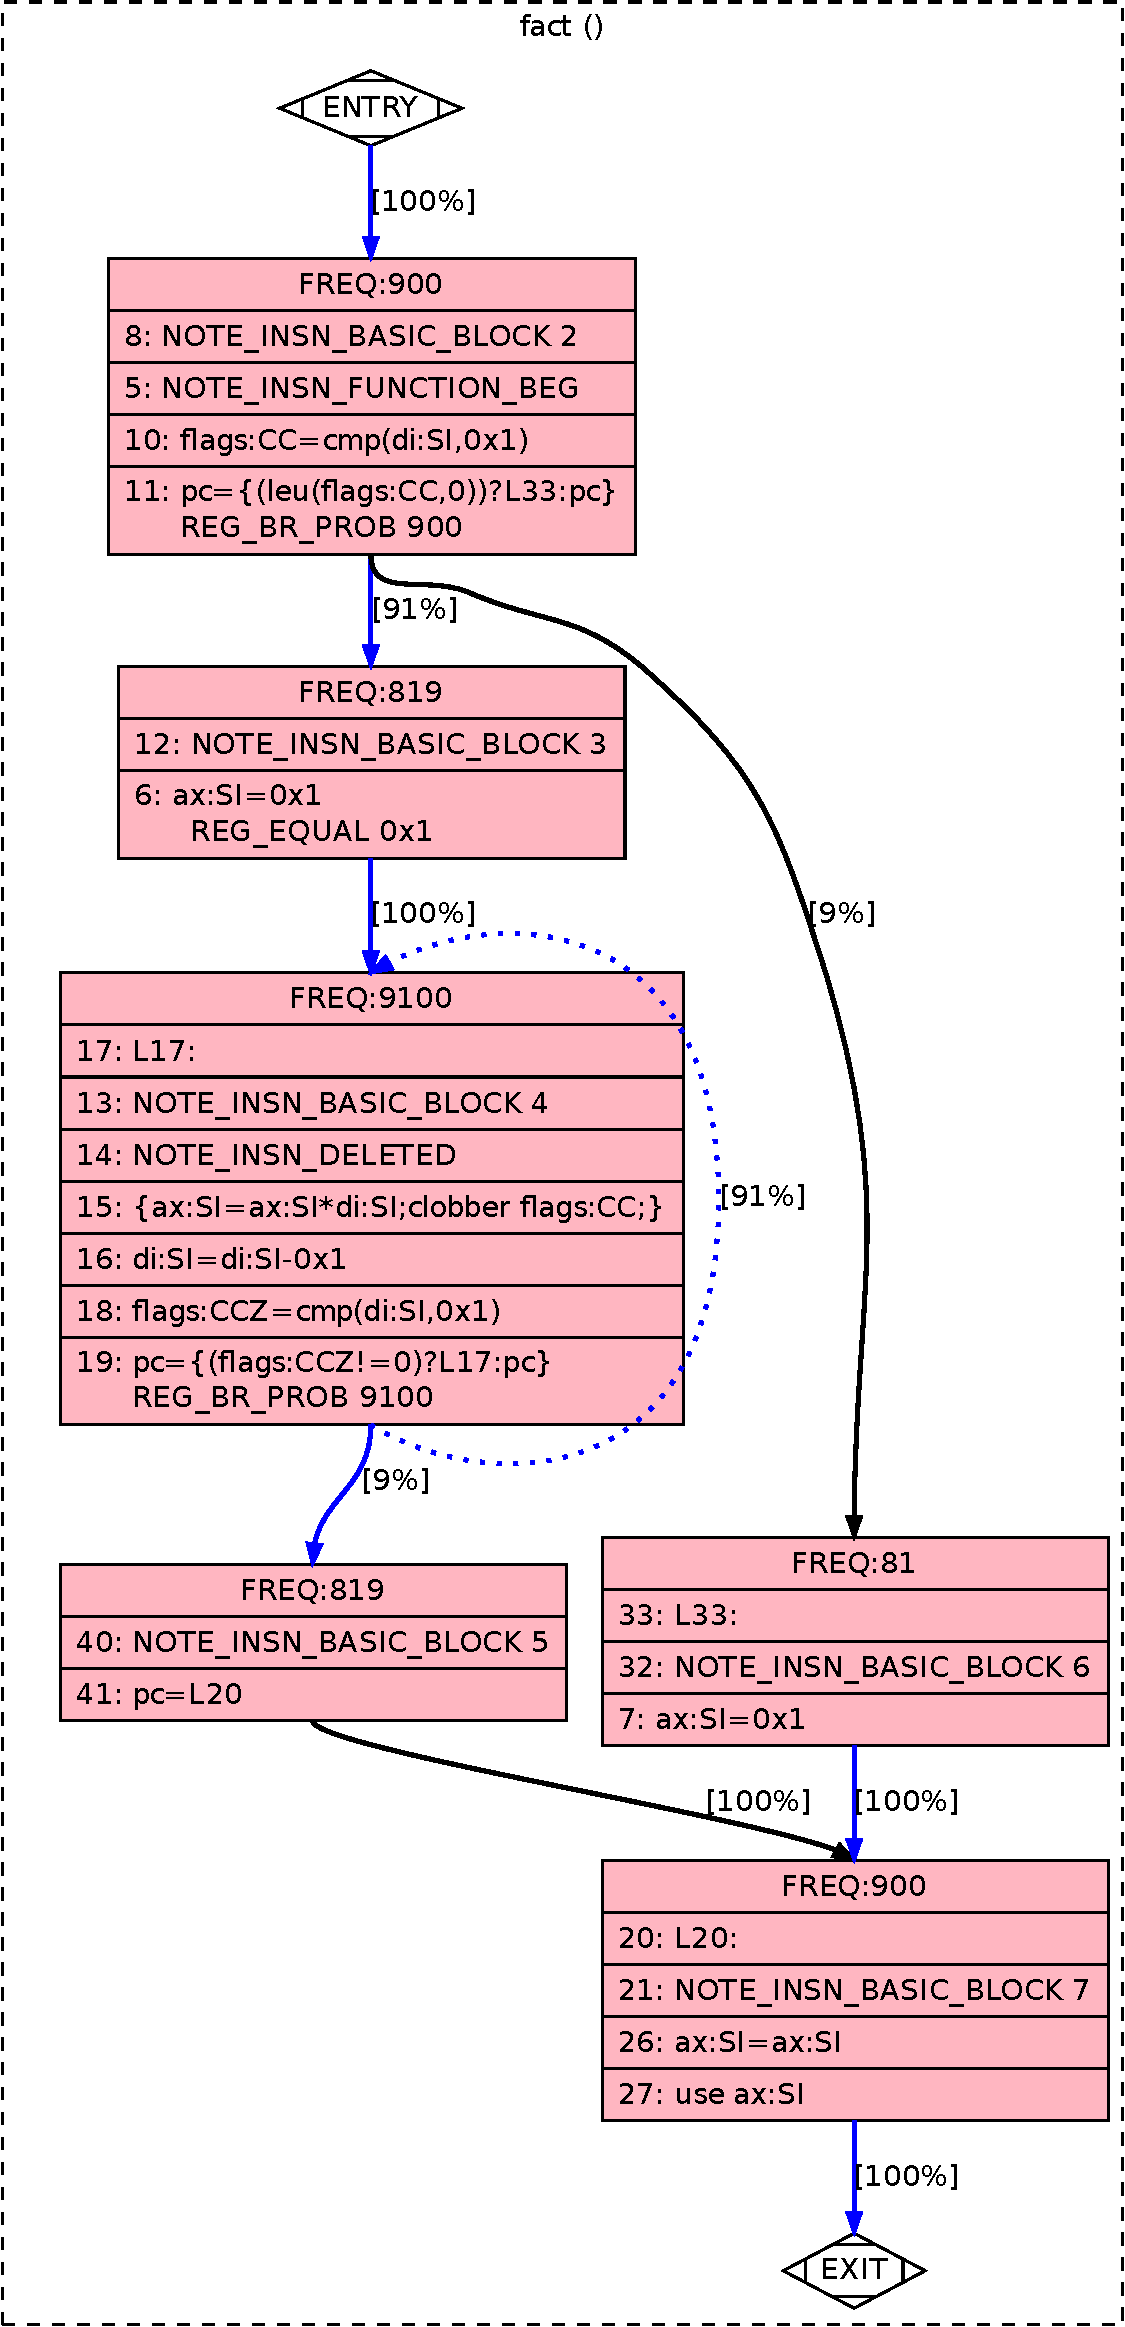
\includegraphics[height=0.7\textheight]{illustrations/fact-reloaded-crop.pdf}
\caption{RTL с физическими регистрами}
\label{fig:fact_rtl_reload}
\end{figure}

После отработки оптимизаций на физических регистрах (if-conversion, переупорядочение базовых блоков, расписание инструкций), кодогенератор в GCC порождает ассемблер целевой архитектуры.

В других компиляторах детали происходящего могут отличаться: в LLVM машинно-независимый IR очень похож на машинно-зависимый, в ICC промежуточное представление скрыто от пользователя и так далее. Но общая схема везде одна и та же: выскоуровневый IR (обычно машинно-независимый) преобразуется в машинно-зависимый IR среднего уровня, который после распределения регистров преобразуется в низкоуровневый IR. Который, в свою очередь, уже и используется для генерации кода.

\pagebreak
\subsection{Ассемблер}

Важно различать язык ассемблера как язык и ассемблер как программу. Язык ассемблера целевой архитектуры задается документом, который называется Instruction Set Architecture (ISA) и является своим для каждой архитектуры. Более того, даже в пределах одной архитектуры могут существовать несколько синтаксисов ассемблера (пример -- AT\&T и Intel синтаксисы ассемблера x86).

\subsubsection{Ассемблирование}

Ассемблер как программа обрабатывает текстовый файл на языке ассемблера конкретной архитектуры и порождает объектный код для последующей линковки и исполнения.

В качестве примера, ассемблер (x86, синтаксис AT\&T), порождённый из функции факториал может выглядеть следующим образом:

\begin{verbatim}
  .file "fact.c"
  .section  .text.unlikely,"ax",@progbits
.LCOLDB0:
  .text
.LHOTB0:
  .p2align 4,,15
  .globl  fact
  .type fact, @function
fact:
.LFB0:
  .cfi_startproc
  cmpl  $1, %edi
  movl  $1, %eax
  jbe .L4
  .p2align 4,,10
  .p2align 3
.L3:
  imull %edi, %eax
  subl  $1, %edi
  cmpl  $1, %edi
  jne .L3
  rep; ret
.L4:
  rep; ret
  .cfi_endproc
.LFE0:
  .size fact, .-fact
\end{verbatim}

В нём можно выделить: 

\begin{itemize}
\item Инструкции x86: \lstinline!cmpl!, \lstinline!movl!, \lstinline!jbe!, \lstinline!imull!, \lstinline!subl! и прочие
\item Метки: \lstinline!fact!, \lstinline!LFB0!, \lstinline!L3!, \lstinline!L4!, \lstinline!LFE0!
Можно заметить, что одна из этих меток -- \lstinline!fact! объявлена глобальной, то есть попадёт в таблицу экспортируемых из этого модуля функций
\item Директивы: \lstinline!globl!, \lstinline!type!, \lstinline!size!, \lstinline!p2align!
\item Отладочную информацию: \lstinline!cfi_startproc!, \lstinline!cfi_endproc!
\item Секции \lstinline!text!, \lstinline!text.unlikely!
\end{itemize}

Ассемблер выполняет следующую работу:

\begin{enumerate}
\item Кодирование инструкций
\item Подстановка абсолютных значений переходов (где они известны) вместо символьных меток
\item Ассемблирование секций (кода, данных, стека)
\item Исполнение директив ассемблера (выравнивание, отладочная информация, прочее)
\item Формирование таблиц экспорта
\end{enumerate}

\subsubsection{Макроассемблер}

Почти любой ассемблер (включая ml.exe от Microsoft, GNU AS, а также отдельные распространённые ассемблеры, такие как wasm и nasm) поддерживает не только свои основные функции по обработке выдачи компилятора, но также предоставляет определенные средства для разработки собственно на языке ассемблера. В современном мире чистая разработка на ассемблере это экзотика, но она может быть нужна для работы с системными регистрами, использовании специфичных возможностей архитектуры и так далее -- в общем для всего, чего нельзя написать на C.

Препроцессор ассемблера обычно позволяет:

\begin{itemize}
\item Объявлять и использовать макросы. Например приведенный ниже макрос для GNU AS:

\begin{verbatim}
.macro  sum from=0, to=5
  .long   \from
  .if     \to-\from
  sum     "(\from+1)",\to
  .endif
.endm
\end{verbatim}

При вызове \lstinline!SUM 0,5! раскроется в:
 
\begin{verbatim}
  .long   0
  .long   1
  .long   2
  .long   3
  .long   4
  .long   5
\end{verbatim}

\item Включать ассемблерный код из других файлов (директива \lstinline!.include "file"! в GNU as или аналогичные ей).
\item Писать комментарии. Стили комментирования очень разнообразны и отличаются от ассемблера к ассемблеру. Большинство ассемблеров также поддерживают комментарии в стиле C.
\item Также поддерживаются дополнительные (иногда -- удивительно разнообразные) возможности. Так например в GNU as символ точка обозначает адрес текущей ассемблируемой инструкции. Поэтому запись:

\begin{verbatim}
melvin: .long .
\end{verbatim}

Обозначает, что метка melvin содержит собственный адрес.
\end{itemize}

Кроме общих для всех архитектур возможностей ассемблера в рамках его синтаксиса, каждая архитектура может определять набор своих средств для задания адресов в памяти, обращения к регистрам и так далее.

\subsubsection{Дизассемблирование}

Результатом работы ассемблера является объектный файл, который, в свою очередь, может быть дизассемблирован, то есть переведен обратно в ассемблерное представление. В случае GNU toolchain соответствующая утилита называется objdump. 

\begin{verbatim}
$ as fact.s -o fact.o
$ objdump -d fact.o
\end{verbatim}

Ниже рассмотрен вывод ассемблированного и сразу же дизассемблированного кода:

\begin{verbatim}
   0:	83 ff 01             	cmp    $0x1,%edi
   3:	b8 01 00 00 00       	mov    $0x1,%eax
   8:	76 13                	jbe    1d <fact+0x1d>
   a:	66 0f 1f 44 00 00    	nopw   0x0(%rax,%rax,1)
  10:	0f af c7             	imul   %edi,%eax
  13:	83 ef 01             	sub    $0x1,%edi
  16:	83 ff 01             	cmp    $0x1,%edi
  19:	75 f5                	jne    10 <fact+0x10>
  1b:	f3 c3                	repz retq 
  1d:	f3 c3                	repz retq 
\end{verbatim}

Дизассемблер аннотирован кодировкой (ниже будут рассмотрены способы аннотировать дизассемблер многим другим, в том числе номерами строк и даже самими строчками исходного кода программы).

Кроме того видно, что две p2align директивы породили выравнивающий nop.

\pagebreak
\subsection{Линкер}

Линкер это программа, предназначенная для связывания (linking) нескольких объектных файлов в один исполняемый. Линкер входит во все известные наборы средств разработки -- в случае GCC или LLVM он называется ld (или gold, это улучшенная версия ld от Google), в случае Microsoft это link.exe, есть и другие варианты линкеров.

\subsubsection{Объявления и определения}

Прежде чем переходить к рассмотрению линкера, необходимо расширить тестовую задачу. Пусть функция \lstinline!fact! физически находится в файле \lstinline!fact.c! и кроме него есть файл \lstinline!main.c! следующего содержимого:

\begin{lstlisting}
int
main (void)
{
  printf ("%d\n", fact(5));
  return 0;
}
\end{lstlisting}

Но откуда вообще компилятор при обработке этого фйла узнает что такое \lstinline!fact! и что такое \lstinline!printf!?

Простейший способ скомпилировать их вместе это подать оба файла программе-драйверу:

\begin{verbatim}
$ gcc main.c fact.c
\end{verbatim}

Но что и в каком порядке при этом будет сделано?



\end{document}
